%====================================================================================
\section[Producción]{Externalidades de producción}
%====================================================================================

\begin{frame}{Externalidades de producción}
Se definen:
	\begin{itemize}
		\item Costo Marginal Privado $(CMgP)$ o Costo marginal $(CMg)$ = costo de los factores de producción.
		\item Externalidad $(Ext)$ o Costo Externo marginal $(CEMg)$ = aumento del costo impuesto externamente cuando una o más empresas aumentan su producción en una unidad.
		\item Costo Marginal Social $(CMgS)$ o Costo Social marginal $(CSMg)= CMg + CEMg$.
	\end{itemize}
\end{frame}
%------------------------------------------------
\begin{frame}{Externalidades de producción}
		\begin{center}
		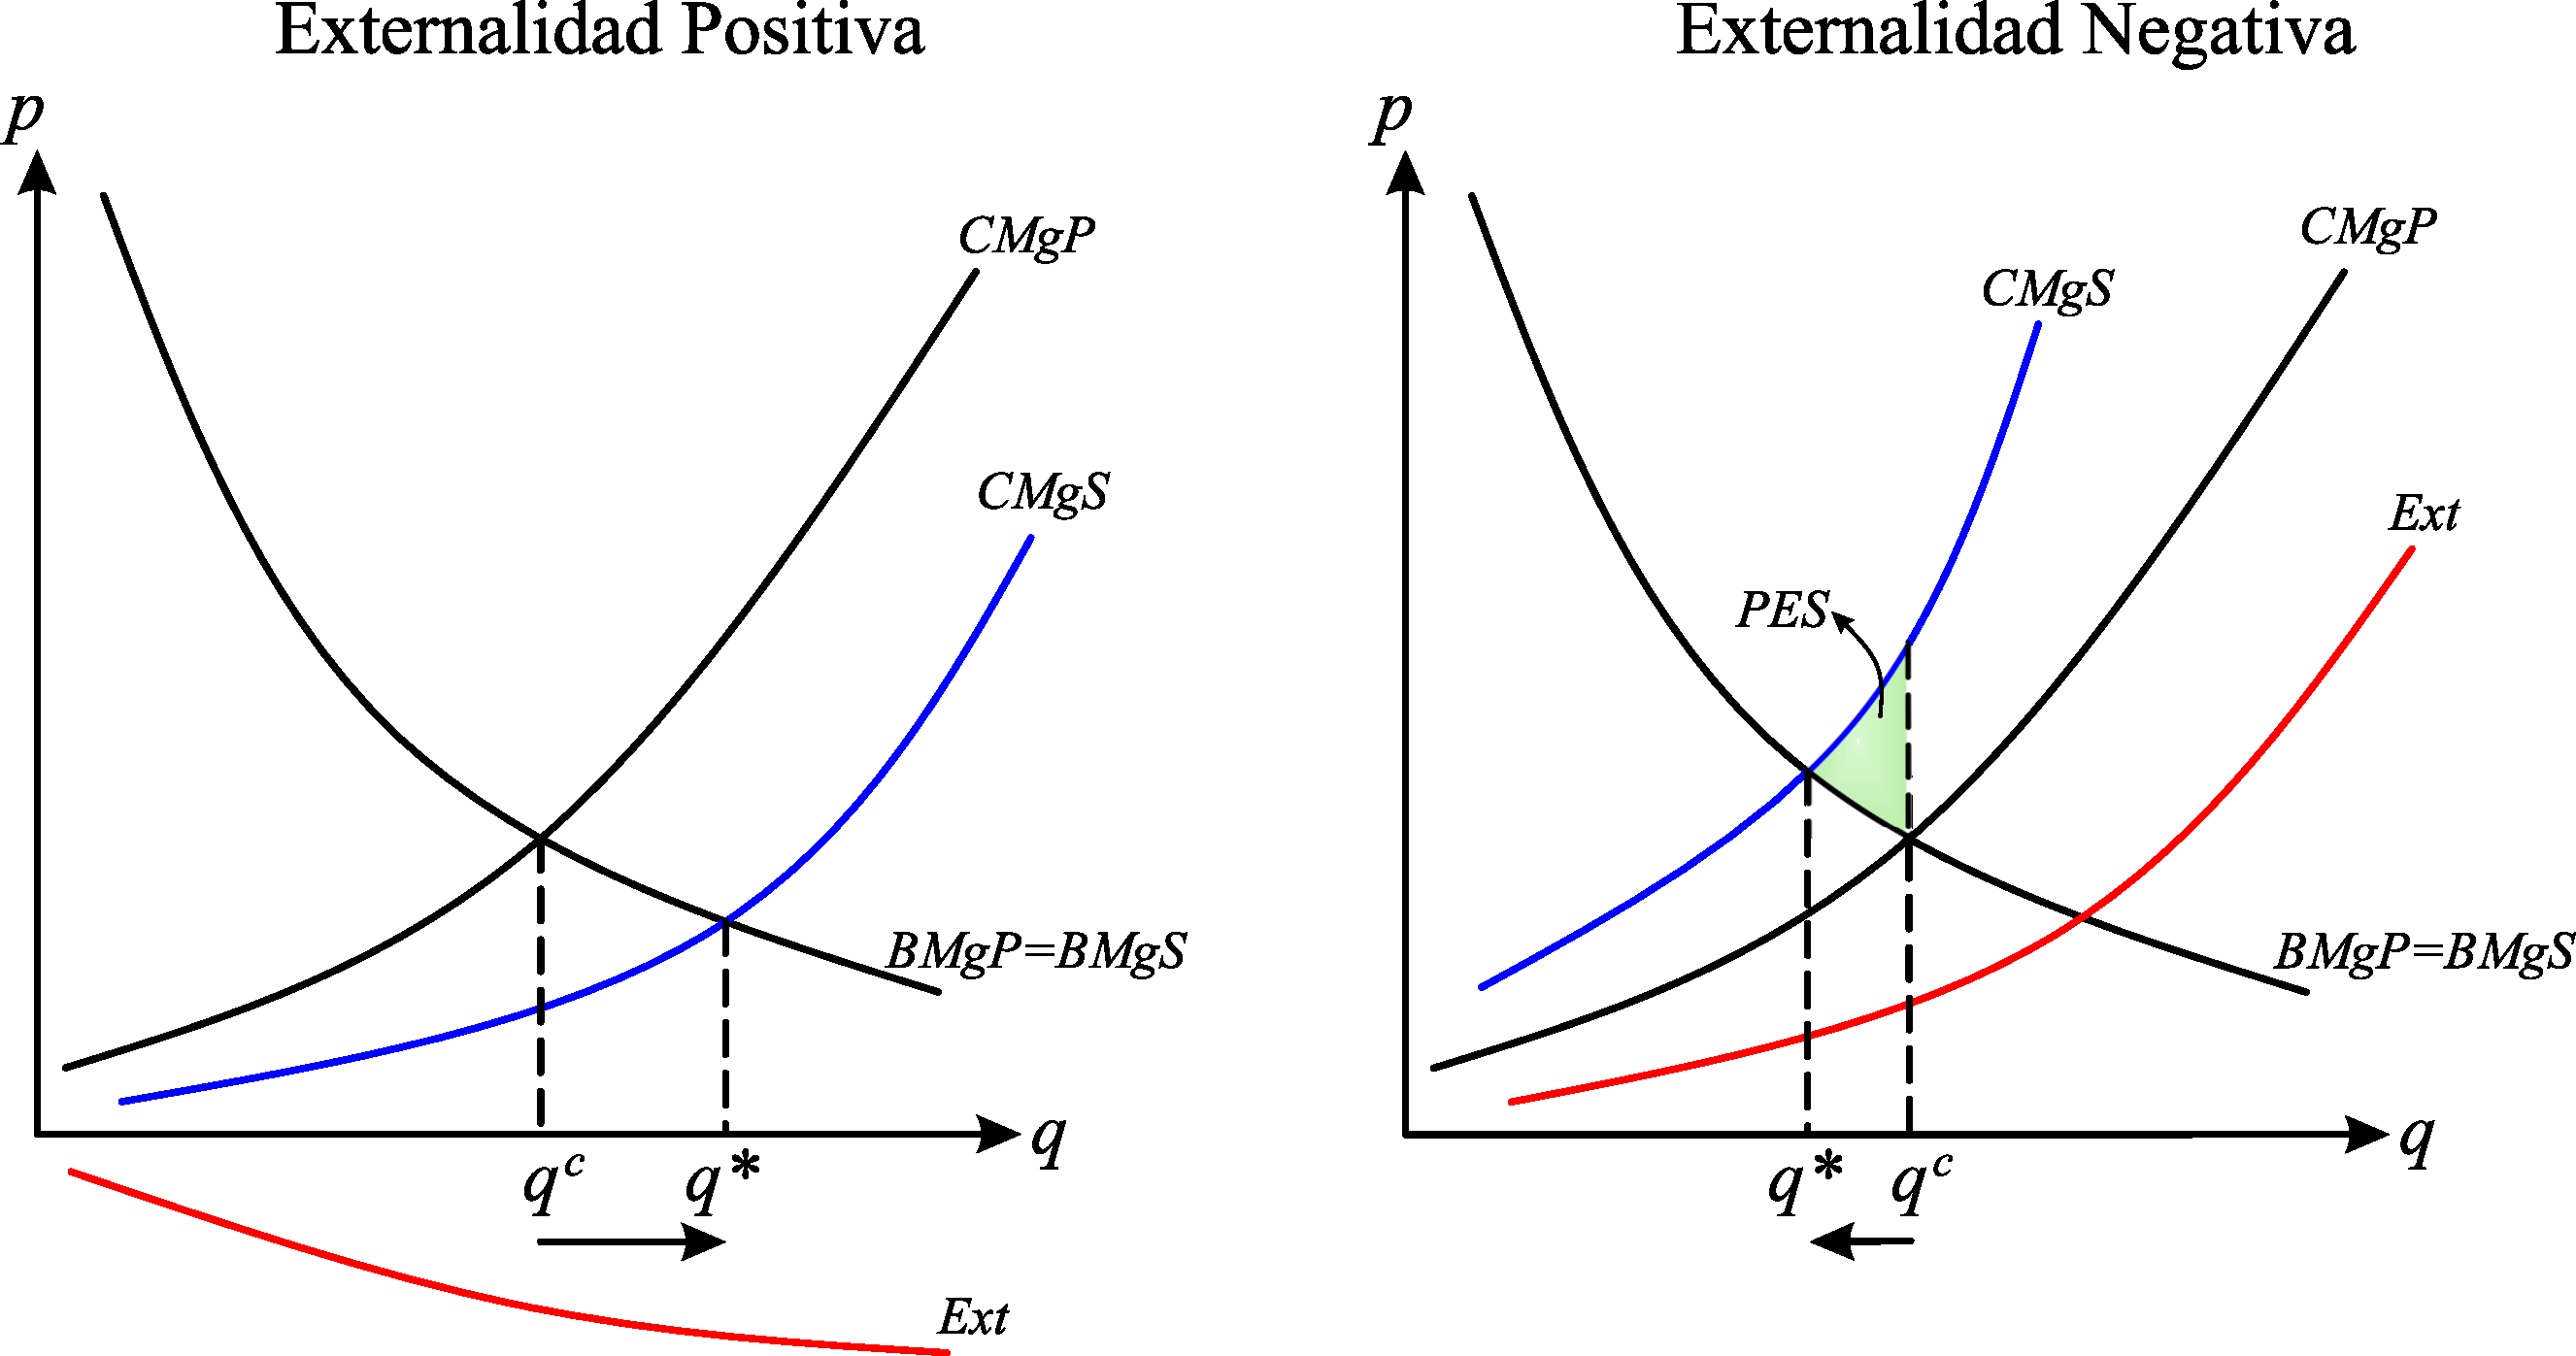
\includegraphics[width = 1\linewidth]{figures/produccion.pdf}
	\end{center}
\end{frame}
%------------------------------------------------
\begin{frame}{Externalidades de producción}
	\begin{itemize}
		\item Sean dos empresas: una acería $(S)$ y una piscigranja $(F)$.
		\item La empresa $S$ produce
			\begin{itemize}
				\item $s$ cantidad de acero
				\item $x$ cantidad de contaminación que se vierte a un río contiguo.
			\end{itemize}
		\item La empresa $F$ produce
			\begin{itemize}
				\item $f$ cantidad de pescado
			\end{itemize}
		\item La empresa $F$ se encuentra río abajo y se perjudica por la contaminación de la empresa $S$.
		\item Las funciones de costo son:
			\begin{itemize}
				\item Para S: $c_s(s,x)$
				\item Para F: $c_f(f,x)$
			\end{itemize}
	\end{itemize}
\end{frame}
%------------------------------------------------
\begin{frame}{Externalidades de producción}
	Supuestos
		\begin{itemize}
			\item La mayor contaminación eleva el costo de la producción de pescado
					$$\frac{\partial c_f}{\partial x} > 0$$
			\item La reducción del nivel de contaminación, elevará el costo de producción de acero
					$$\frac{\partial c_s}{\partial x} \leq 0$$
		\end{itemize}
\end{frame}
%------------------------------------------------
\begin{frame}{Problemas de maximización de beneficio}
	\begin{itemize}
		\item Para la acería: 
				$$\M \limits_{s,x} \pi_s = p_ss - c_s(s,x)$$
			  La acería elige la producción de acero y de contaminación que maximice su $\pi$.
		\item Para la piscigranja: 
				$$\M \limits_{f}\pi_f = p_f - c_f(f,x)$$
		      La piscigranja sólo determina cantidad de pescado, no controla la contaminación.
	\end{itemize}
\end{frame}
%------------------------------------------------
\begin{frame}{Problemas de maximización de beneficio}
	\begingroup
		\setlength{\tabcolsep}{10pt} % Default value: 6pt
		\renewcommand{\arraystretch}{1.5} % Default value: 1
			\begin{tabular}{ccc}
				\hline
					Para la acería & {} & Para la piscigranja\\
					$\M \limits_{s,x} \pi_s = p_ss - c_s(s,x)$ & {} & $\M \limits_{f} \pi_f = p_f - c_f(f,x)$\\
				\hline 
					\multicolumn{3}{c}{condiciones de primer orden} \\
				\hline
					$\frac{\partial \pi}{\partial s} = 0 \Leftrightarrow p_s - \frac{\partial c_s(s^\ast,x^\ast)}{\partial s} = 0$ & {} & $\frac{\partial \pi}{\partial f} = 0 \Leftrightarrow p_f - \frac{\partial c_f(f^\ast,x^\ast)}{\partial f} = 0$\\
					$p_s = \frac{\partial c_s(s^\ast,x^\ast)}{\partial s}$ & {} & $p_f = \frac{\partial c_f(f^\ast,x^\ast)}{\partial f}$\\
					$\frac{\partial \pi}{\partial x} = 0 \Leftrightarrow - \frac{\partial c_s(s^\ast,x^\ast)}{\partial x} = 0$ &{} & {}\\
					$0 = \frac{\partial c_s(s^\ast,x^\ast)}{\partial x}$& {} & {} \\
				\hline
			\end{tabular}
	\endgroup
\end{frame}
%------------------------------------------------
\begin{frame}{Problemas de maximización de beneficio}
	Interpretación
		\begin{itemize}
			\item La acería produce acero donde precio = $CMg$ de producir dicho acero.
					$$p_s = \frac{\partial c_s(s^\ast,x^\ast)}{\partial s}$$
			\item Y genera desechos donde el $CMg$ de producirlos es nulo.
					$$0 = \frac{\partial c_s(s^\ast,x^\ast)}{\partial x}$$
			\item La piscifactoría produce donde precio de pescado = CMg de producir pescado.
					$$p_f = \frac{\partial c_f(f^\ast,x^\ast)}{\partial f}$$
		\end{itemize}
\end{frame}
%------------------------------------------------
\begin{frame}{¿Por qué hay externalidad?}
	\begin{itemize}
		\item La acería produce demasiada contaminación, porque no le cuesta hacerlo.
		\item La cantidad óptima de acero sólo considera su costo de producción, no el daño que ocasiona a la piscigranja. 
		\item Como la piscigranja no puede controlar la cantidad de desecho que genera la acería, debe incurrir en mayores costos para eliminar el desecho del agua.
	\end{itemize}
\end{frame}
%------------------------------------------------
\begin{frame}{La solución eficiente}
	Fusionarse y maximizar el beneficio conjunto:
			$$\pi_s + \pi_f = p_ss - c_s(s,x) + p_ff - c_f(f,x)$$
				\vspace{-0.4cm}
		\begin{itemize}
			\item La empresa conjunta tiene en cuenta ahora los costos de todos los agentes ( costos de la producción de acero +  daño que le produce a la piscicultura). 
			\item Si: 
					$$\pi = p_ss + p_ff - c_s(s,x) - c_f(f,x)$$
			\item Las CPO son:
					\begin{gather*}
						\frac{\partial \pi}{\partial s} = 0 \Leftrightarrow p_s - \frac{\partial c_s(s^\ast,x^\ast)}{\partial s} = 0 \Leftrightarrow p_s - \frac{\partial c_S}{\partial s} - \frac{\partial c_f}{\partial x} \cdot \frac{\partial x}{\partial s} = 0\\
						p_s =  \frac{\partial c_s}{\partial s} + \frac{\partial c_f}{\partial x} \cdot \frac{\partial x}{\partial s}
					\end{gather*}
		\end{itemize}
\end{frame}
%------------------------------------------------
\begin{frame}{Gráficamente}
Por tanto, la producción óptima social de acero será menor a la producción privada.
	\begin{center}
		\begin{tikzpicture}[scale=1]
	% Formación de la caja
	% Consumidor A
	\draw[->] (0.5,0.5) node[align=center, below left] {\footnotesize $O_A$} -- (0.5,4.5) node[align=center, above] {\footnotesize $x_{2}^{A}$};
	\draw[->] (0.5,0.5) -- (8.5,0.5) node[align=center, right] {\footnotesize $x_{1}^{A}$};
	
	\draw (6,0.5) node[below] {\footnotesize $x_{1}^{A}$};
	\draw (0.5,2) node[left] {\footnotesize $x_{2}^{A}$};
	
	% Llaves
	\draw [decorate,decoration={brace,amplitude=5pt},xshift=-4pt,yshift=0pt] (6.1,-0.05) -- (0.7,-0.05);
	\node [right] at (3,-0.4) {$w_{1}^{A}$};
	
	\draw [decorate,decoration={brace,amplitude=5pt},xshift=-4pt,yshift=0pt] (-0.05,0.5) --(-0.05,2);
	\node [left] at (-0.3,1.27) {$w_{2}^{A}$};
\end{tikzpicture}
	\end{center}
\end{frame}
%------------------------------------------------
\begin{frame}{La solución eficiente}
	\begin{center}
		\begingroup
		\setlength{\tabcolsep}{10pt} % Default value: 6pt
		\renewcommand{\arraystretch}{1.5} % Default value: 1
			\begin{tabular}{p{4cm}cp{4cm}}
				\hline
					\multicolumn{3}{c}{Si: $\pi= p_ss + p_ff - c_s(s,x) - c_f(f,x)$} \\
				\hline
					Las CPO son: &{}&\\
				\hline
					$\frac{\partial \pi}{\partial x} = 0 \Leftrightarrow -\frac{\partial c_S}{\partial x} - \frac{\partial c_f}{\partial x} = 0$ &{}& $\frac{\partial \pi}{\partial f} \Leftrightarrow p_f - \frac{\partial c_f}{\partial f} = 0$\\
					$-\frac{\partial c_s}{\partial x} = \frac{\partial c_f}{\partial x}$ &{}& $p_f = \frac{\partial c_f}{\partial f}$\\
					&{}& Como la actividad de la piscigranja no ejerce externalidad, el óptimo privado es igual al óptimo social. \\
				\hline
			\end{tabular}
		\endgroup
	\end{center}
\end{frame}
%------------------------------------------------
\begin{frame}{Gráficamente}
La acería producirá menos desecho que antes porque enfrenta un costo positivo al contaminar, frente al costo nulo de antes.
	\begin{center}
		\vspace{-0.5cm}
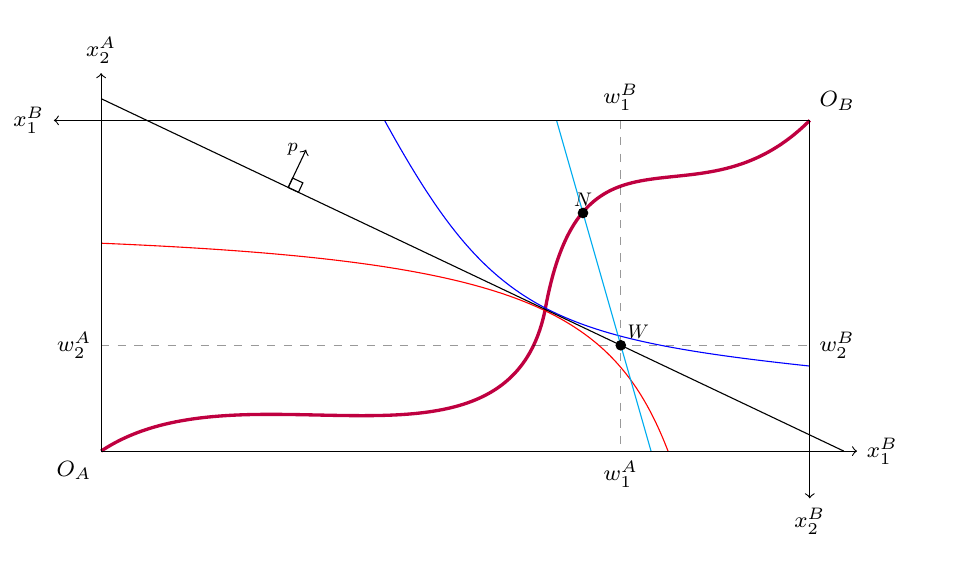
\begin{tikzpicture}[scale=1.2]
	\hspace{-0.3cm}
	% Curva de contrato 5.2,2
		\draw  [purple, very thick] (0.5,0.5) ..controls (2,1.5) and (4.8,0) .. (5.2,2) ..controls (5.6,4.2) and (6.8,2.8) .. (8,4);
	% Intersección de una dotación
		% Oferta: w
			\draw[dashed, opacity=0.4] (6,4) node [above, opacity=1] {\footnotesize $w_{1}^{B}$} -- (6,0.5) node [below, opacity=1] {\footnotesize $w_{1}^{A}$};
			\draw[dashed, opacity=0.4] (0.5,1.62)  node [left, opacity=1] {\footnotesize $w_{2}^{A}$} -- (8,1.62) node [right, opacity=1] {\footnotesize $w_{2}^{B}$};
	
	% Curvas de indiferencia
		\draw [blue] (3.5,4) .. controls (4.6,2) and (5.2,1.7) .. (8,1.4);
		\draw [red] (0.5,2.7) .. controls (4.915,2.515) and (5.915,2.015) .. (6.5,0.5);
	
	% Recta presupuestaria
		\draw (0.5,4.23) -- (8.36,0.5);
		\draw [cyan](5.32,4) -- (6.32,0.5);
		
	% Flecha y rectángulo
		\draw [->] (2.48,3.29) -- (2.67,3.69) node [left, scale = 0.3mm] {\footnotesize $p$};
		\draw [rotate around={-25:(2.48,3.29)}] (2.48,3.29) rectangle (2.6, 3.4);
	
	% Puntos
		\draw[black, fill=black] (5.6,3.02) circle[radius=0.05] node [above, scale=0.25mm] {$N$};
		\draw[black, fill=black] (6,1.62) circle[radius=0.05] node [above right, scale=0.25mm] {$W$};
	
	% Formación de la caja
		% Consumidor A
			\draw[->] (0.5,0.5) node[align=center, below left] {\footnotesize $O_A$} -- (0.5,4.5) node[align=center, above] {\footnotesize $x_{2}^{A}$};
			\draw[->] (0.5,0.5) -- (8.5,0.5) node[align=center, right] {\footnotesize $x_{1}^{B}$};
			
		%Consumidor B
			\draw[->] (8,4) node[align=center, above right] {\footnotesize $O_B$} -- (0,4) node[align=center, left] {\footnotesize $x_{1}^{B}$};
			\draw[->] (8,4) -- (8,0) node[align=center, below] {\footnotesize $x_{2}^{B}$};
\end{tikzpicture}
	\end{center}
\end{frame}